\documentclass{article}

\usepackage[italian]{babel}
\usepackage[margin=2cm, footskip=5mm]{geometry}
% questi package non sono necessari in lualatex; ref https://tex.stackexchange.com/a/413046
% \usepackage[utf8]{inputenc}
% \usepackage[T1]{fontenc}
\usepackage{enumitem}
\usepackage{hyperref}
\usepackage{titlesec}
\usepackage{soulutf8}
\usepackage{contour}
\usepackage{float}
\usepackage{graphicx}
\usepackage{fancyhdr}
\usepackage{longtable}
\usepackage[table]{xcolor}
\usepackage{titling}
\usepackage{lastpage}
\usepackage{ifthen}
\usepackage{calc}
\usepackage{minted}
\usepackage{pgfgantt}
\usepackage{subfiles}

\newlength{\imgwidth}

\newcommand\scalegraphics[1]{%
    \settowidth{\imgwidth}{\includegraphics{#1}}%
    \setlength{\imgwidth}{\minof{\imgwidth}{\textwidth}}%
    \includegraphics[width=\imgwidth]{#1}%
}

% XXX definizione dei percorsi in cui cercare immagini
\graphicspath{ {./}
    {./img/}
}

% esempio di utilizzo: \appendToGraphicspath{./img/} (un comando diverso per ogni path da includere)
% N.B.: ci DEVE essere un forward slash alla fine del path, a indicare che è una cartella.
\makeatletter
\newcommand\appendToGraphicspath[1]{%
  \g@addto@macro\Ginput@path{{#1}}%
}
\makeatother

% setup della sottolineatura
\setuldepth{Flat}
\contourlength{0.8pt}

\newcommand{\uline}[1]{%
  \ul{{\phantom{#1}}}%
  \llap{\contour{white}{#1}}%
}

% setup dei link
\hypersetup{
  colorlinks=true, % set true if you want colored links
  linktoc=all,     % set to all if you want both sections and subsections linked
  linkcolor=black, % choose some color if you want links to stand out
}

% setup di header e footer
\pagestyle{fancy}

\fancyhf{}
\fancyhead[L]{\includegraphics[width=1cm]{logo.png}}
\fancyhead[R]{\thetitle}
\fancyfoot[R]{\thepage\ di~\pageref{LastPage}}

\fancypagestyle{nopage}{%
  \fancyfoot{}%
}

\setlength{\headheight}{1.2cm}

% setup forma \paragraph e \subparagraph
\titleformat{\paragraph}[hang]{\normalfont\normalsize\bfseries}{\theparagraph}{1em}{}
\titleformat{\subparagraph}[hang]{\normalfont\normalsize\bfseries}{\thesubparagraph}{1em}{}

% setup profondità indice di default
\setcounter{secnumdepth}{5}
\setcounter{tocdepth}{5}

% shortcut per i placeholder
\newcommand{\plchold}[1]{\textit{\{#1\}}} % chktex 20

% hook per lo script che genera il glossario
\newcommand{\glossario}[1]{\underline{#1}\textsubscript{g}}

% definizione dei comandi \uso e \stato
\makeatletter
\newcommand{\setUso}[1]{%
  \newcommand{\@uso}{#1}%
}
\newcommand{\uso}{\@uso}

\newcommand{\setStato}[1]{%
  \newcommand{\@stato}{#1}%
}
\newcommand{\stato}{\@stato}

\newcommand{\setVersione}[1]{%
  \newcommand{\@versione}{#1}%
}
\newcommand{\versione}{\@versione}

\newcommand{\setResponsabile}[1]{%
  \newcommand{\@responsabile}{#1}%
}
\newcommand{\responsabile}{\@responsabile}

\newcommand{\setRedattori}[1]{%
  \newcommand{\@redattori}{#1}%
}
\newcommand{\redattori}{\@redattori}

\newcommand{\setVerificatori}[1]{%
  \newcommand{\@verificatori}{#1}%
}
\newcommand{\verificatori}{\@verificatori}

\newcommand{\setDescrizione}[1]{%
  \newcommand{\@descrizione}{#1}%
}
\newcommand{\descrizione}{\@descrizione}

\newcommand{\setModifiche}[1]{%
  \newcommand{\@modifiche}{#1}%
}

\newcommand{\modifiche}{\@modifiche}

\makeatother

% setup delle description
\setlist[description,1]{font=$\bullet$\hspace{1.5mm}, labelwidth=* leftmargin=*,labelindent=12.5mm}
\setlist[description,2]{font=$\bullet$\hspace{1.5mm}, leftmargin=*,labelindent=12.5mm}

\appendToGraphicspath{../../commons/img/}

\title{Verbale esterno --- 17/02/2020}

\setResponsabile{Alessandro Rizzo}
\setRedattori{Alberto Cocco}
\setVerificatori{
  Tobia Apolloni \\ &
  Riccardo Cestaro \\ &
  Fabio Scettro
}
\setUso{Esterno}
\setDescrizione{Verbale dell'incontro di GruppOne del 17/02/2019}
\setModifiche{%
\cellcolor{white!80!lightgray!100} & Alessandro Rizzo & 2020--02--18 & approva documento \\%
\cellcolor{white!80!lightgray!100} & Verificatori & 2020--02--18 & verifica verbale \\%
\multirow{-3}{*}{-} \cellcolor{white!80!lightgray!100} & Alberto Cocco & 2020--02--17 & stendi verbale %
}

\disabilitaVersione{}
\disabilitaElencoFigure{}
\disabilitaElencoTabelle{}

\begin{document}

\thispagestyle{empty}
\pagenumbering{gobble}

\begin{center}

  \includegraphics[width=8.5cm]{\commons/img/logo.png}\\
  {\Large GruppOne - progetto "Stalker"}\\
  \vspace{1.5cm}

  {\Huge \thetitle}
  \vspace{1.5cm}

  \begin{table}[H]
    \centering

    \begin{tabular}{r|l}
      \textbf{Versione}     & \versione              \\
      \textbf{Approvazione} & \responsabile          \\
      \textbf{Redazione}    & \redattori             \\
      \textbf{Verifica}     & \verificatori          \\
      \textbf{Stato}        & \stato                 \\
      \textbf{Uso}          & \uso                   \\
      \textbf{Destinato a}  & Imola Informatica      \\
                            & GruppOne               \\
                            & Prof. Tullio Vardanega \\
                            & Prof. Riccardo Cardin  \\
    \end{tabular}
  \end{table}

  \vspace{3cm}
  \textbf{Descrizione}\\
  \descrizione\\
  \vfill
  \verb|gruppone.swe@gmail.com|
\end{center}

\newpage
\thispagestyle{nopage}

\section*{Registro delle modifiche}
\label{sec:registro_delle_modifiche}

\begin{table}[H]
  \label{tab:registro_delle_modifiche}

  \centering
  \rowcolors{2}{lightgray}{white!80!lightgray!100}

  \begin{longtable}[c]{c c c c l}
    \rowcolor{darkgray!90!}\color{white}{\textbf{Versione}} & \color{white}{\textbf{Data}} & \color{white}{\textbf{Nominativo}} & \color{white}{\textbf{Ruolo}} & \color{white}{\textbf{Descrizione}} \\\endhead
    \modifiche
  \end{longtable}
\end{table}

% section registro_delle_modifiche (end)
\newpage

\thispagestyle{nopage}
\pagenumbering{roman}
\tableofcontents

\newpage

\pagenumbering{arabic}


\section{Informazioni logistiche}%
\label{sec:informazioni_logistiche}

\begin{description}
  \item [Luogo] Torre Archimede, ufficio del Professor Tullio Vardanega
  \item [Data] 17/02/2020
  \item [Ora] 10:00 \symbol{8594} 11:00
\end{description}

\subsection{Membri del gruppo presenti}%
\label{sub:membri_del_gruppo_presenti}

\begin{enumerate}
  \item Riccardo Agatea
  % \item Tobia Apolloni
  % \item Riccardo Cestaro
  \item Alberto Cocco
  \item Luca Ercole
  \item Alberto Gobbo
  \item Alessandro Rizzo
  % \item Fabio Scettro
\end{enumerate}
% sub:membri_del_gruppo_presenti (end)

\subsection{Altri partecipanti}%
\label{sub:altri_partecipanti}

\begin{enumerate}
  \item Prof.\ Tullio Vardanega (committente)
\end{enumerate}

% sub:altri_partecipanti (end)
% sec:informazioni_logistiche (end)

\section{Introduzione}%
\label{sec:introduzione}

L'incontro ci è servito per risolvere dubbi e avere chiarimenti riguardo alle indicazioni del Professore sui documenti consegnati in precedenza per la revisione dei requisiti.

\section{Ordine del giorno}%
\label{sec:ordine_del_giorno}

\begin{itemize}
  \item Lettere accentate
  \item Chiarimenti su Piano di progetto e modalità di consegna
  \item Registro delle modifiche
  \item Metriche per la qualità di prodotto e piano di qualifica
  \item Rapporto col proponente.
\end{itemize}

\section{Lettere accentate}%
\label{sec:lettere_accentate}

\textbf{Domanda:} Cosa intende con codifica degli accenti non corretti all'interno delle norme di progetto e del piano di qualifica? \\
\textbf{Risposta:} Il professore ci ha rammentato l'esistenza di due tipi di accento in italiano.
Dobbiamo, quindi, riflettere maggiormente su come codificare gli accenti perché ha riscontrato delle irregolarità in alcuni documenti.
% sec:lettere_accentate (end)

\section{Chiarimenti Piano di progetto e modalità di consegna}%
\label{sec:piano_di_progetto_e_modalita_di_consegna}

\textbf{Domanda:} Per l'invio della versione corretta, cosa intende con ``invio formale di documentazione correttiva''?
Dobbiamo consegnare tutti i documenti come in entrata alla RR (con cartella drive ecc.), anche se ovviamente gli altri documenti non sono ancora corretti, oppure possiamo inviargli solo il Piano di progetto?
Nel secondo caso, con che modalità (allegato a email, cartella drive con solo quello dentro, …)?\\
\textbf{Risposta:} Il Professore ci ha assicurato che per risolvere la non conformità basta inviare il PdP corretto.
Tuttavia, non sarebbe intelligente eseguire una rettifica solo economica ma è necessaria anche una nuova riflessione sulla pianificazione che permetta di avere un PdP sufficientemente fatto bene entro la prossima e imminente revisione di progettazione.
Inoltre, per consegnare il documento corretto si deve fornire al Professore un puntatore al repo che contiene il PdP aggiornato.

\subsection{Addendum su piano di progetto}%
\label{sub:addendum_su_piano_di_progetto}

Successivamente il Professore ha ribadito l'importanza di effettuare un riallineamento del Piano di Progetto a livello logico che deve quindi pianificare anche la realizzazione di un PoC (Proof of Concept) e di una successiva PB (Product Baseline) di cui non ha trovato alcun riscontro nei PdP dei gruppi che hanno consegnato alla prima revisione dei requisiti.
Il PoC, infatti, serve per fare pratica con le tecnologie che abbiamo scelto di impiegare e richiede un'attenta pianificazione.
Probabilmente ne realizzeremo un certo numero, mentre al Professor Cardin ne mostreremo solo uno.
A tal proposito è fondamentale non creare sin da subito delle distorsioni tra ciò che realmente stiamo facendo e ciò che abbiamo pianificato nel Piano di progetto.
Il nostro obiettivo è di redigere un Piano di progetto che possa essere un libro mastro che ci dice quante ore abbiamo disponibili e quante ne possiamo ancora spendere.
In sostanza il PdP deve cercare di riflettere il più possibile il vero evitando di avere troppi scostamenti a consuntivo che vanno in qualche modo a minarne l'efficacia.
Proprio per facilitare il lavoro di pianificazione il Professore ci ha suggerito di creare degli intervalli di plausibilità in cui assegnare l'impegno di lavoro del gruppo.
Il consuntivo deve essere realizzato a posteriori e serve come strumento di verifica.
Il Professore, inoltre, ha osservato che sarebbe desiderabile avere i dati del PdP all'interno del repo e che il piano di progetto venga prodotto in corrispondenza delle revisioni che non devono essere viste come degli obiettivi da soddisfare ma come dei vincoli che abbiamo l'obbligo di rispettare.
Gli obiettivi settimanali e le modalità con cui decidiamo di organizzare il lavoro spettano unicamente a noi.
Per questa ragione ci è stato consigliato di realizzare dei resoconti settimanali per verificare se stiamo lavorando come quanto pianificato o se è necessario redistribuire il lavoro.
Ovviamente il Professore non è interessato a tali resoconti, che vanno però regolamentati all'interno delle Norme di Progetto.

% sub:addendum_su_piano_di_progetto (end)
% sec:piano_di_progetto_e_modalita_di_consegna (end)
\section{Registro delle modifiche}%
\label{sec:registro_modifiche}

\textbf{Domanda:} Nel registro delle modifiche, non va bene avere più azioni associate allo stesso numero di versione.
Vuol dire che dobbiamo cambiare il modo in cui gestiamo il numero di versione?
Oppure che il numero di versione va bene, ma allora non ha senso metterlo nel registro delle modifiche?\\
\textbf{Risposta:} Il Professore ci ha comunicato che nella scelta del numero di versione siamo stati esplorativi rispetto agli altri gruppi e che ha però avuto delle osservazioni di presentazione.
Ogni modifica al repo, infatti, avviene in seguito ad una catena di eventi: realizzazione, verifica e approvazione.
L'incremento di versione deve, quindi, avvenire in corrispondenza di un cambiamento all'interno del repository.
Nel nostro caso lo scatto di versione avviene sin dalla prima modifica riportata all'interno del registro delle modifiche e ciò non ha alcun senso.
È quindi fondamentale avere un processo che monitori le modifiche che avvengono ed è importante che ad ogni nuovo numero di versione corrisponda la concatenazione di eventi che ha comportato lo scatto di versione.

% sec:registro_delle modifiche (end)
\section{Metriche per la qualità di prodotto e piano di qualifica}%
\label{sec:metriche_per_la_qualita_di_prodotto_e_piano_di_qualifica}

\textbf{Domanda:} A quale processo/attività competono le metriche di qualità di prodotto?\\
\textbf{Risposta:} Il Professore ci ha ricordato che le norme devono contenere i processi che abbiamo deciso di istanziare e le metriche che abbiamo deciso di utilizzare per valutare la qualità.
Il PdQ deve invece andare a definire dei valori soglia per ogni metrica.
Associare ogni metrica di prodotto alla corrispondente attività di processo nelle norme non è un esercizio banale.

\textbf{Domanda:} Le metriche sono relative ad attività e non a processi, corretto? Quindi per ogni attività c'è un paragrafo metrica innestato\\
\textbf{Risposta:} Le metriche vanno sempre associate alle rispettive attività.
I processi sono come dei contenitori astratti che servono semplicemente per raggruppare le attività.
% sec:metriche_per_la_qualita_di_prodotto_e_piano_di_qualifica (end)

\newpage
\section{Registro delle decisioni}%
\label{sec:registro_delle_decisioni}

\begin{description}
  \item[20200217-ext-001] Modificare il sistema dei numeri di versione e registro delle modifiche.
  \item[20200217-ext-002] Semplificare e normare l'attività di compilazione del consuntivo di periodo.
\end{description}

% sec:registro_delle_decisioni (end)

\end{document}
